\chapter*{Dodatak: Prikaz aktivnosti grupe}
		\addcontentsline{toc}{chapter}{Dodatak: Prikaz aktivnosti grupe}
		
		\section*{Dnevnik sastajanja}
		
		\begin{packed_enum}
			\item  sastanak
			\item[] \begin{packed_item}
				\item Datum: 14. listopada 2020.
				\item Prisustvovali: cijeli PreljevStoga
				\item Teme sastanka:
				\begin{packed_item}
					\item  diskusija zadatka
					\item  upoznavanje s git-om i GitLab-om
				\end{packed_item}
			\end{packed_item}
			
			\item  sastanak
			\item[] \begin{packed_item}
				\item Datum: 15. listopada 2020.
				\item Prisustvovali: dr.sc.M.Krhen, I.Rissi, cijeli PreljevStoga
				\item Teme sastanka:
				\begin{packed_item}
					\item  diskutiranje zadatka koji si je grupa zadala
					\item  savjeti za rad na projektu
				\end{packed_item}
			\end{packed_item}
			
			\item  sastanak
			\item[] \begin{packed_item}
				\item Datum: 22. listopada 2020.
				\item Prisustvovali: dr.sc.M.Krhen, I.Rissi, D.Grubelić, J.Komljenović, A.Lakoš, L.Pranjić, M.Vladić
				\item Teme sastanka:
				\begin{packed_item}
					\item  upit vezan uz ispravno pisanje dokumentacije
				\end{packed_item}
			\end{packed_item}
			
			\item  sastanak
			\item[] \begin{packed_item}
				\item Datum: 24. listopada 2020.
				\item Prisustvovali: cijeli PreljevStoga
				\item Teme sastanka:
				\begin{packed_item}
					\item  odabir tehnologija
					\item  raspoređivanje poslova
					\item  definiranje zadataka za naredni tjedan
				\end{packed_item}
			\end{packed_item}
			
			\item  sastanak
			\item[] \begin{packed_item}
				\item Datum: 28. listopada 2020.
				\item Prisustvovali: T.Bjelčić, D.Grubelić, J.Komljenović, A.Lakoš, L.Pranjić, M.Vladić
				\item Teme sastanka:
				\begin{packed_item}
					\item  demonstracija prve inačice dokumentacije
					\item  definiranje strukture git \textit{repositoryja} i raščišćavanje drugih nedoumica oko git-a
					\item  priprema za izradu temeljne inačice Android dijela aplikacije
					\item  definiranje daljnjeg rasporeda poslova
				\end{packed_item}
			\end{packed_item}
			
			\item  sastanak
			\item[] \begin{packed_item}
				\item Datum: 29. listopada 2020.
				\item Prisustvovali: D.Grubelić, J.Komljenović, A.Lakoš
				\item Teme sastanka:
				\begin{packed_item}
					\item  demonstracija rada s djangom J.Komljenovića
				\end{packed_item}
			\end{packed_item}
			
			\item  sastanak
			\item[] \begin{packed_item}
				\item Datum: 29. listopada 2020.
				\item Prisustvovali: dr.sc.M.Krhen, I.Rissi, T.Bjelčić, D.Grubelić, J.Komljenović, A.Lakoš, L.Pranjić, M.Vladić
				\item Teme sastanka:
				\begin{packed_item}
					\item  dogovor oko izmjene funkcionalnih zahtjeva
					\item  upit vezan uz pravilan izgled UML dijagrama
				\end{packed_item}
			\end{packed_item}
			
			\item  sastanak
			\item[] \begin{packed_item}
				\item Datum: 1. studenog 2020.
				\item Prisustvovali: T. Bjelčić, D.Grubelić, J.Komljenović, A.Lakoš, M.Vladić
				\item Teme sastanka:
				\begin{packed_item}
					\item  demonstracija napretka na backend dijelu
					\item  dogovor oko daljnjeg rasporeda poslova
				\end{packed_item}
			\end{packed_item}
			
			\item  sastanak
			\item[] \begin{packed_item}
				\item Datum: 2. studenog 2020.
				\item Prisustvovali: T.Bjelčić, D.Grubelić, J.Komljenović, A.Lakoš, L.Pranjić, M.Vladić
				\item Teme sastanka:
				\begin{packed_item}
					\item  rasprava o budućim planovima s obzirom na zadaće iz drugog predmeta
					\item  dogovor o prebacivanju SQL upita o artiklima i trgovinama na poslužitelj
				\end{packed_item}
			\end{packed_item}
			
			\item  sastanak
			\item[] \begin{packed_item}
				\item Datum: 6. studenog 2020.
				\item Prisustvovali: cijeli PreljevStoga
				\item Teme sastanka:
				\begin{packed_item}
					\item  dogovor oko opsega generičkih funkcionalnosti za prvu predaju
					\item  raspored poslova
					\item  kratki prolazak kroz dokumentaciju
				\end{packed_item}
			\end{packed_item}
			
			\item  sastanak
			\item[] \begin{packed_item}
				\item Datum: 7. studenog 2020.
				\item Prisustvovali: cijeli PreljevStoga
				\item Teme sastanka:
				\begin{packed_item}
					\item  priprema za prvu predaju
				\end{packed_item}
			\end{packed_item}
			
			\item  sastanak
			\item[] \begin{packed_item}
				\item Datum: 13. prosinca 2020.
				\item Prisustvovali: cijeli PreljevStoga
				\item Teme sastanka:
				\begin{packed_item}
					\item  raspored poslova nakon prve predaje
				\end{packed_item}
			\end{packed_item}
			
			\item  sastanak
			\item[] \begin{packed_item}
				\item Datum: 23. prosinca 2020.
				\item Prisustvovali: cijeli PreljevStoga
				\item Teme sastanka:
				\begin{packed_item}
					\item  komunikacija poslužitelja i androida
				\end{packed_item}
			\end{packed_item}
			
			\item  sastanak
			\item[] \begin{packed_item}
				\item Datum: 28. prosinca 2020.
				\item Prisustvovali: cijeli PreljevStoga
				\item Teme sastanka:
				\begin{packed_item}
					\item  prikaz podataka na Androidu
				\end{packed_item}
			\end{packed_item}
			
			\item  sastanak
			\item[] \begin{packed_item}
				\item Datum: 2. siječnja 2020.
				\item Prisustvovali: cijeli PreljevStoga
				\item Teme sastanka:
				\begin{packed_item}
					\item  implementacija prijave pomoću Google računa
				\end{packed_item}
			\end{packed_item}
			
			\item  sastanak
			\item[] \begin{packed_item}
				\item Datum: 8. siječnja 2020.
				\item Prisustvovali: cijeli PreljevStoga
				\item Teme sastanka:
				\begin{packed_item}
					\item  priprema za testiranje
				\end{packed_item}
			\end{packed_item}
			
			\item  sastanak
			\item[] \begin{packed_item}
				\item Datum: 12. siječnja 2020.
				\item Prisustvovali: cijeli PreljevStoga
				\item Teme sastanka:
				\begin{packed_item}
					\item  priprema za drugu predaju
				\end{packed_item}
			\end{packed_item}
			
			%
			
		\end{packed_enum}
		
		\eject
		\section*{Tablica aktivnosti}
		    \begin{longtabu} to \textwidth {|X[7, l]|X[1, c]|X[1, c]|X[1, c]|X[1, c]|X[1, c]|X[1, c]|X[1, c]|}
								
				\cline{2-8} \multicolumn{1}{c|}{\textbf{}} &     \multicolumn{1}{c|}{\rotatebox{90}{\textbf{Tomislav Bjelčić }}} & \multicolumn{1}{c|}{\rotatebox{90}{\textbf{Dominik Brdar }}} &	\multicolumn{1}{c|}{\rotatebox{90}{\textbf{Damjan Grubelić }}} &	\multicolumn{1}{c|}{\rotatebox{90}{\textbf{Josip Komljenović }}} &
				\multicolumn{1}{c|}{\rotatebox{90}{\textbf{Antonio Lakoš }}} &
				\multicolumn{1}{c|}{\rotatebox{90}{\textbf{Luka Pranjić }}} &	\multicolumn{1}{c|}{\rotatebox{90}{\textbf{Marko Vladić }}} \\ \hline 
				\endfirsthead
				
			
				\cline{2-8} \multicolumn{1}{c|}{\textbf{}} &     \multicolumn{1}{c|}{\rotatebox{90}{\textbf{Tomislav Bjelčić}}} & \multicolumn{1}{c|}{\rotatebox{90}{\textbf{Dominik Brdar }}} &	\multicolumn{1}{c|}{\rotatebox{90}{\textbf{Damjan Grubelić }}} &
				\multicolumn{1}{c|}{\rotatebox{90}{\textbf{Josip Komljenović }}} &	\multicolumn{1}{c|}{\rotatebox{90}{\textbf{Antonio Lakoš }}} &
				\multicolumn{1}{c|}{\rotatebox{90}{\textbf{Luka Pranjić }}} &	\multicolumn{1}{c|}{\rotatebox{90}{\textbf{Marko Vladić }}} \\ \hline 
				\endhead
				
				
				\endfoot
							
				 
				\endlastfoot
				
				Upravljanje projektom 		& 5 &  & 3 & 2 & 25 & 3 & \\ \hline
				Opis projektnog zadatka 	& 6 & 1 & 3 &  & 12 & 5 & 2 \\ \hline
				
				Funkcionalni zahtjevi       & 5 & 1 & 2 & 3 & 2 & 3 & 2 \\ \hline
				Opis pojedinih obrazaca 	&  &  & 24 &  & 3 &  &  \\ \hline
				Dijagram obrazaca 			&  & 1 & 5 &  & 3 & 2 &  \\ \hline
				Sekvencijski dijagrami 		&  & 2 & 4 &  &  &  &  \\ \hline
				Opis ostalih zahtjeva 		&  & 2 & 1 &  & 2 &  & 1 \\ \hline

				Arhitektura i dizajn sustava	 & 2 & 2 & 8 &  & 15 & 4 & 2 \\ \hline
				Baza podataka				&  & 3 & 4 & 5 & 14 &  &   \\ \hline
				Dijagram razreda 			&  &  &  &  &  & 4 &  2 \\ \hline
				Dijagram stanja				&  &  &  &  & 1 &  &  \\ \hline
				Dijagram aktivnosti 		&  &  &  &  & 1 &  &  \\ \hline
				Dijagram komponenti			&  &  &  &  & 1 &  &  \\ \hline
				Korištene tehnologije i alati 		& 4 & 4 &  &  & 1 & 7 &  2\\ \hline
				Ispitivanje programskog rješenja 	& 5 & 12 & 4 & 36 & 45 & 18 & 16 \\ \hline
				Dijagram razmještaja			&  &  &  &  & 1 &  &  \\ \hline
				Upute za puštanje u pogon 		&  & 2 & 4 &  & 1 &  &  \\ \hline 
				Dnevnik sastajanja 			& 3 & 1 & 2 &  & 1 &  & 1 \\ \hline
				Zaključak i budući rad 		&  &  &  &  &  & 6 &  \\  \hline
				Popis literature 			&  &  & 1 &  &  &  &  \\  \hline
				Demonstracija nove tehnologije &  &  & 3 &  & 1 &  &  \\ \hline
				Back end     		        &  & 13 & 2 & 30 & 95 & 2 & 18 \\ \hline 
				Dizajn sučelja              & 8 & 7 & 4 & 1 & 2 & 6 & 5 \\ \hline
				Front end              & 19 & 13 & 24 & 3 & 15 & 21 & 23 \\ \hline
				
				
			\end{longtabu}
					
					
		\eject
		\section*{Dijagrami pregleda promjena}
			\begin{figure}[H]
				\centering
				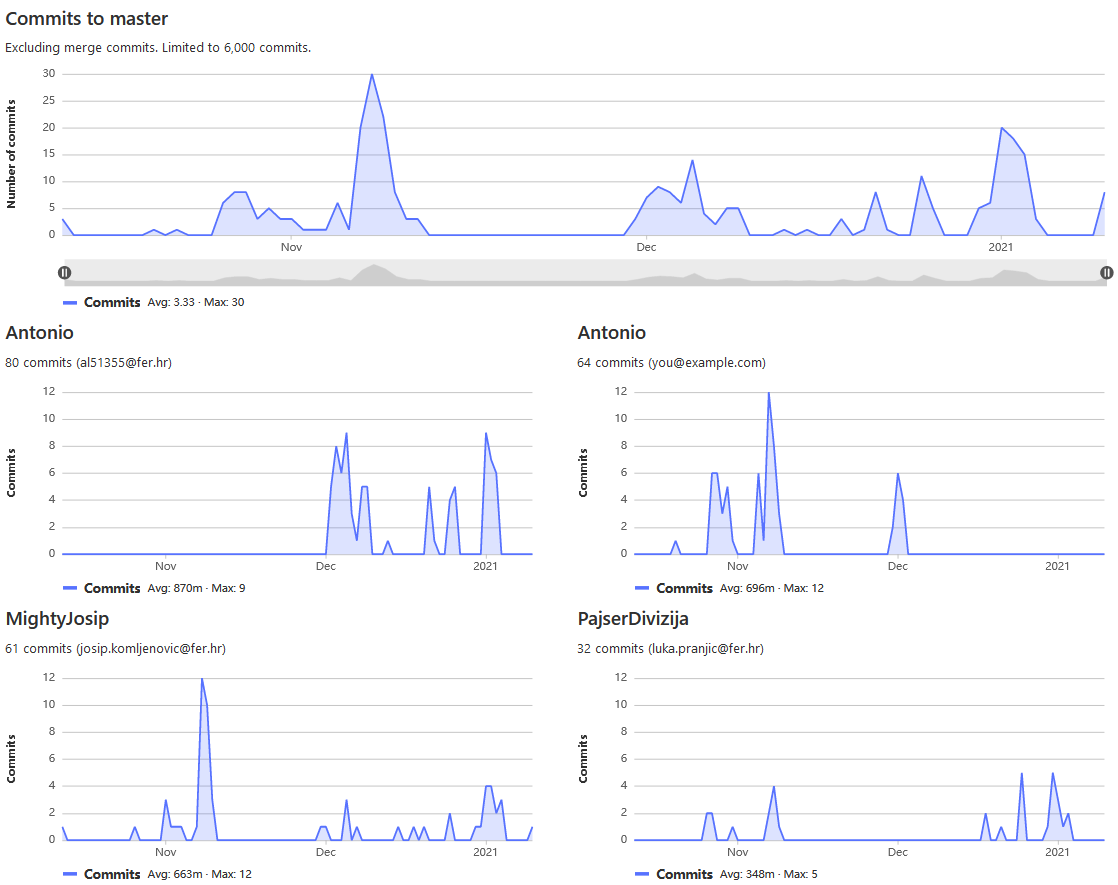
\includegraphics[scale=0.5]{slike/DijagramPromjena1.png}
				\caption{Dijagram pregleda promjena 1}
				\label{fig:dij_pregled_promjena1}
			\end{figure}
			\begin{figure}[H]
				\centering
				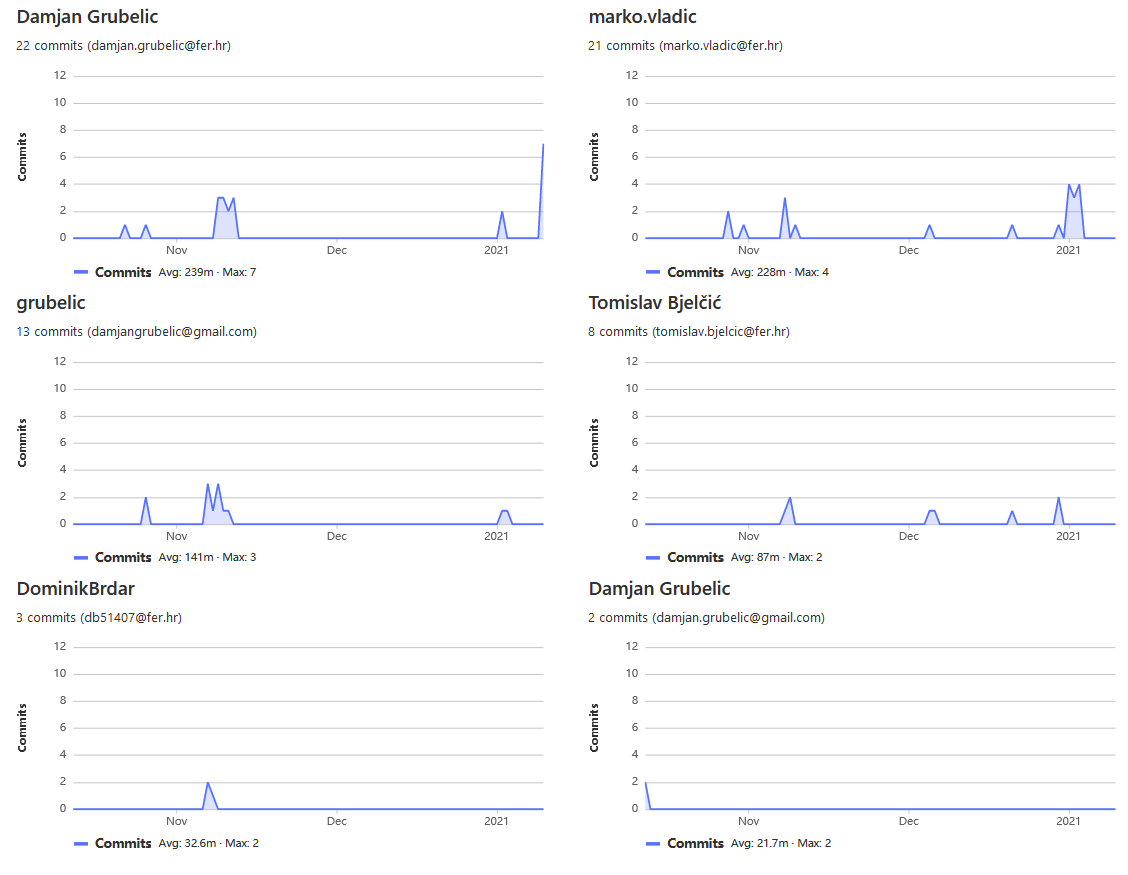
\includegraphics[scale=0.5]{slike/DijagramPromjena2.png}
				\caption{Dijagram pregleda promjena 2}
				\label{fig:dij_pregled_promjena2}
			\end{figure}
			
	
